\documentclass[hyperref={pdfpagelabels=false}]{beamer}
\usetheme[block=fill]{metropolis}

\usepackage[portuguese]{babel}
\usepackage[utf8]{inputenc} % To use characters such as é without typing é
\usepackage{ctable}
\usepackage{listings}
\lstset{%
  language=Matlab,
  showstringspaces=false,
  basicstyle=\linespread{0.9}\ttfamily,
  keywordstyle=\textbf,
  commentstyle=\color{gray},
  stringstyle=\color{orange},
  numbers=left,
  numberstyle=\tiny\color{gray},
  stepnumber=1,
  numbersep=10pt,
  columns=fullflexible,
  tabsize=3,
  frame=single,
  frameround=tttt
}
\let\Tiny=\tiny % eliminates compilation errors
\usepackage{fontspec}

\title{Laboratório de Matemática Computacional II}
\subtitle{Aula 3}
\author[M. Weber Mendonça]{Melissa Weber Mendonça\\
Universidade Federal de Santa Catarina}
\date{2011}

\begin{document}
\setmonofont{Inconsolata}

\begin{frame}
  \titlepage
\end{frame}

\begin{frame}{Na aula passada...}
   \begin{center} {\texttt{tril(A)}} \end{center}
   \begin{center} {\texttt{triu(A)}} \end{center}
\end{frame}

\begin{frame}{Exercício}
   Decompor uma matriz em uma soma, na forma
   $$A = U+D+L,$$
   em que $U$ é sua parte triangular superior, $D$ é sua diagonal, e $L$ é sua
   parte triangular inferior.
   \vfill
   \begin{center} \href{listings/split.m}{\underline{\texttt{split.m}}} \end{center}
\end{frame}

\begin{frame}{Reshape}
  \begin{center} {\texttt{reshape(A,tamanho)}} \end{center}
\end{frame}

\begin{frame}{Exercício}
  Criar um vetor aleatório com 24 elementos. Reescrever estes mesmos
  elementos de 4 maneiras diferentes (sem contar as transpostas!)
  \begin{center} \texttt{v = rand(24,1)} \end{center}
  \begin{itemize}
  \item {\texttt{reshape(v,1,24)}} 
  \item {\texttt{reshape(v,2,12)}} 
  \item {\texttt{reshape(v,3,8)}} 
  \item {\texttt{reshape(v,4,6)}} 
  \end{itemize}
\end{frame}

\begin{frame}{Sistemas Lineares}
  \begin{block}{}
	  No estacionamento de um shopping há 8 veículos, entre carros e motos. Sabe-se também que o número de rodas é igual 26. Determine o número de carros e motos.
	\end{block}
	\only<2->{$$x_1 = \mbox{ número de carros }, x_2 = \mbox{ número de motos }$$}
	\only<3>{$$\left\{ \begin{array}{r c r c l} x_1&+&x_2&=&8\\4x_1&+&2x_2&=&26 \end{array} \right.$$}
	\only<4>{$$\left\{ \begin{array}{r c r c l} x_1&+&x_2&=&8\\4x_1&+&2x_2&=&26 \end{array} \right. \Leftrightarrow \begin{array}{r c r c l} x_1&+&x_2&=&8 \alert{\times (-2)}\\4x_1&+&2x_2&=&26 \end{array} $$}
	\only<5>{$$\left\{ \begin{array}{r c r c l} x_1&+&x_2&=&8\\4x_1&+&2x_2&=&26 \end{array} \right. \Leftrightarrow \begin{array}{r c r c l} \alert{-2x_1}&\alert{-}&\alert{2x_2}&\alert{=}&\alert{-16}\\4x_1&+&2x_2&=&26 \end{array}$$}
	\only<6->{$$\left\{ \begin{array}{r c r c l} x_1&+&x_2&=&8\\4x_1&+&2x_2&=&26 \end{array} \right. \Leftrightarrow \begin{array}{r c r c l} -2x_1&-&2x_2&=&-16\\4x_1&+&2x_2&=&26\\\hline 2x_1&&&=&10\end{array}$$}
	\only<7>{$$\Leftrightarrow x_1 = 5$$}
	\only<8>{$$\Leftrightarrow x_1=5, x_2 = 3$$}
\end{frame}

\begin{frame}{Forma matricial}
  \begin{equation*}
    \left\{ 
    \begin{matrix} 
      x_1&+&x_2&=&8\\
      4x_1&+&2x_2&=&26 
    \end{matrix} 
    \right. \Leftrightarrow 
    \begin{bmatrix} 
      1 & 1\\
      4 & 2 
    \end{bmatrix} 
    \begin{bmatrix}
      x_1\\
      x_2
    \end{bmatrix}
    =
    \begin{bmatrix}
      8\\
      26
    \end{bmatrix}
  \end{equation*}
  Chamando 
  \begin{equation*}
    A = \begin{bmatrix} 1&1\\4&2 \end{bmatrix}, x = \begin{bmatrix} x_1\\x_2
    \end{bmatrix} \mbox{ e } b=\begin{bmatrix}8\\26\end{bmatrix},
  \end{equation*}
  podemos escrever o sistema acima como
  $$Ax=b$$
  Assim, a solução será
  \begin{align*}
    x= A^{-1}b &= 
    \begin{bmatrix}
      1 & 1\\
      4 & 2
    \end{bmatrix}^{-1} 
    \begin{bmatrix} 
      8\\
      26 
    \end{bmatrix}
    =
    \begin{bmatrix}
      -1 &1/2\\
      2 & -1/2
    \end{bmatrix}
    \begin{bmatrix} 
      8\\
      26
    \end{bmatrix}
    \\&= 
    \begin{bmatrix}
      -8+26/2\\
      2(8)-26/2
    \end{bmatrix}
    = 
    \begin{bmatrix}
      5\\ 3
    \end{bmatrix}
    .
  \end{align*}
\end{frame}

\begin{frame}{Sistemas Lineares: Solução}
  Se temos um sistema linear dado por
  $$Ax=b$$
  em que $A\in {\mathbb{R}}^{n\times n}$, $x,b \in {\mathbb{R}}^n$ e queremos encontrar $x$, então uma maneira de resolver este problema é fazendo
  $$x = A^{-1}b,$$
  \emph{se a inversa de $A$ existir.}
  \vfill
  No MATLAB, a inversa de $A$ pode ser encontrada se fizermos
  \begin{center}
    {\texttt{inv(A)}}
  \end{center}
\end{frame}

\begin{frame}{Exercício}
  Resolver os sistemas lineares seguintes, usando este método:
  \vfill
  \begin{center} {\texttt{\alert{>>} x = inv(A)*b}} \end{center}
  \vfill
  \begin{itemize}
    \only<1>{\item[1.] $A =
      \begin{pmatrix}
        10 & 1\\
        1 & 1\\
      \end{pmatrix}, b =
      \begin{pmatrix}
        1\\ 1
      \end{pmatrix}$ \qquad $x =
      \begin{pmatrix}
        \alert{-0}\\
        1
      \end{pmatrix}$}
    \only<2>{\item[2.] $A =
      \begin{pmatrix}
        1 & 2 & 3\\
        4 & 5 & 6\\
        7 & 8 & 9
      \end{pmatrix}, b =
      \begin{pmatrix}
        1\\ 2\\ 3
      \end{pmatrix}$ \qquad $x = $??}
    \only<3>{\item[3.] $A =
      \begin{pmatrix}
        1 & 4 & 7\\
        2 & 5 & 8\\
        3 & 6 & 10
      \end{pmatrix}, b =
      \begin{pmatrix}
        1\\ 2\\ 3
      \end{pmatrix}$ \qquad $x =
      \begin{pmatrix}
        1\\
        0\\
        0
      \end{pmatrix}$}
    \only<4>{\item[4.] $A =
      \begin{pmatrix}
        1 & 4 & 7\\
        2 & 5 & 8\\
        2 & 5 & 8
      \end{pmatrix}, b =
      \begin{pmatrix}
        1\\ 2\\ 3
      \end{pmatrix}$ \qquad $x =
      \begin{pmatrix}
        \infty\\
        \infty\\
        \infty
      \end{pmatrix}$ ??}
    \only<5>{\item[5.] $A =
      \begin{pmatrix}
        3 & 17 & 10\\
        2 & 4 & -2\\
        6 & 18 & -12
      \end{pmatrix}, b =
      \begin{pmatrix}
        1\\ 2\\ 3
      \end{pmatrix}$ \qquad $x =
      \begin{pmatrix}
        1.85417\\
        -0.35417\\
        0.14583
      \end{pmatrix}$}
  \end{itemize}
\end{frame}

\begin{frame}{Sistemas Lineares: Regra de Cramer}
  A Regra de Cramer para a resolução de sistemas lineares diz que a solução $x$ de um sistema linear na forma $Ax=b$ pode ser encontrada se fizermos
  $$x_i = \frac{\det(A_i)}{\det(A)},$$
  onde $x = (x_1,\ldots,x_n)$ e $A_i$ é a matriz obtida se substituirmos a coluna $i$ da matriz $A$ pelo lado direito $b$.
  
  Escreva um programa que resolva um sistema linear usando a Regra de Cramer (e dê um aviso, caso $\det(A) = 0$).
  \vfill
  \begin{center} \href{listings/cramer.m}{\underline{\texttt{cramer.m}}} \end{center}
\end{frame}

\begin{frame}{Sistemas Lineares - Gráficos}
  \begin{equation*}
    \left\{ 
    \begin{matrix} 
      x_1&+&x_2&=&8\\
      4x_1&+&2x_2&=&26 
    \end{matrix} 
    \right. \Leftrightarrow 
    \begin{bmatrix} 
      1 & 1\\
      4 & 2 
    \end{bmatrix} 
    \begin{bmatrix}
      x_1\\
      x_2
    \end{bmatrix}
    =
    \begin{bmatrix}
      8\\
      26
    \end{bmatrix}
  \end{equation*}
  Geometricamente...
  \begin{center}
    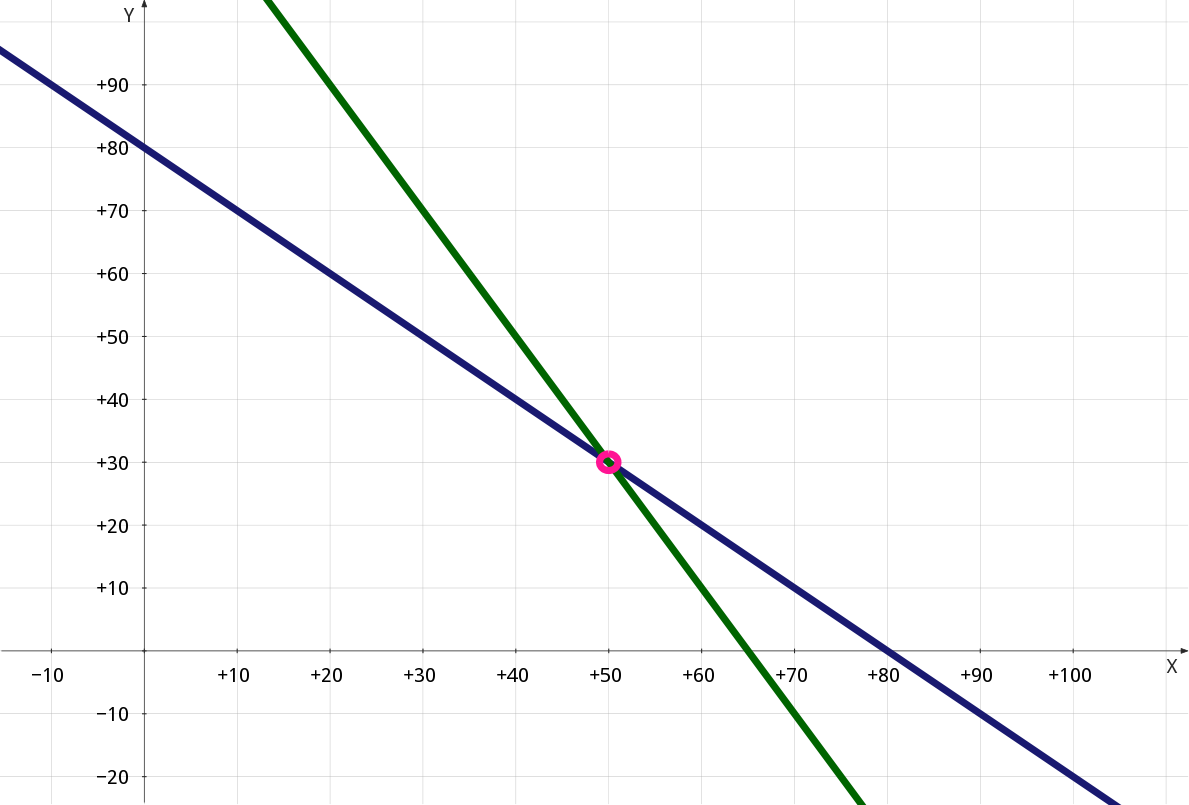
\includegraphics[width=8cm]{img/sistema.png}
  \end{center}
\end{frame}

\begin{frame}{Problemas?}
	$$\left\{ \begin{array}{r c r c l} x&+&y&=&80\\2x&+&2y&=&160 \end{array} \right.$$
	\begin{center}
	  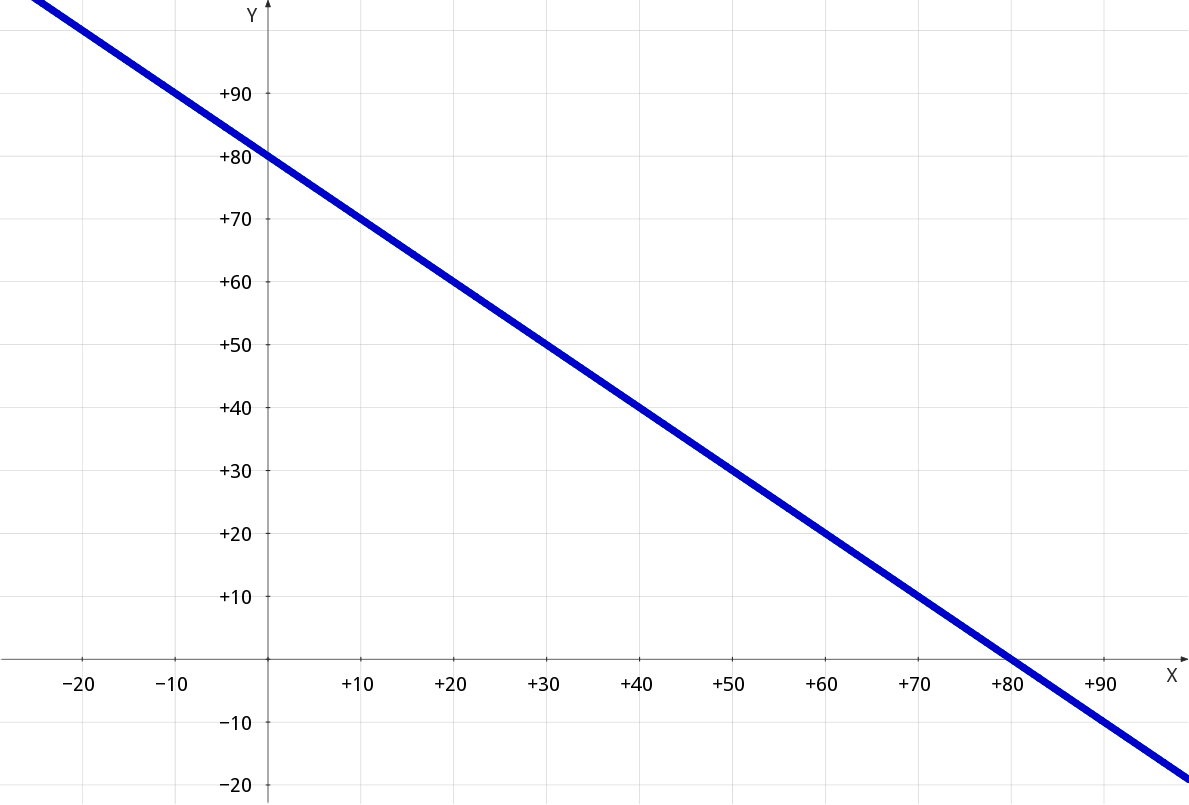
\includegraphics[width=8cm]{img/indeterminado.png}
	\end{center}
\end{frame}

\begin{frame}{Problemas?}
	$$\left\{ \begin{array}{r c r c l} x&+&y&=&80\\2x&+&2y&=&100 \end{array} \right.$$
	\begin{center}
	   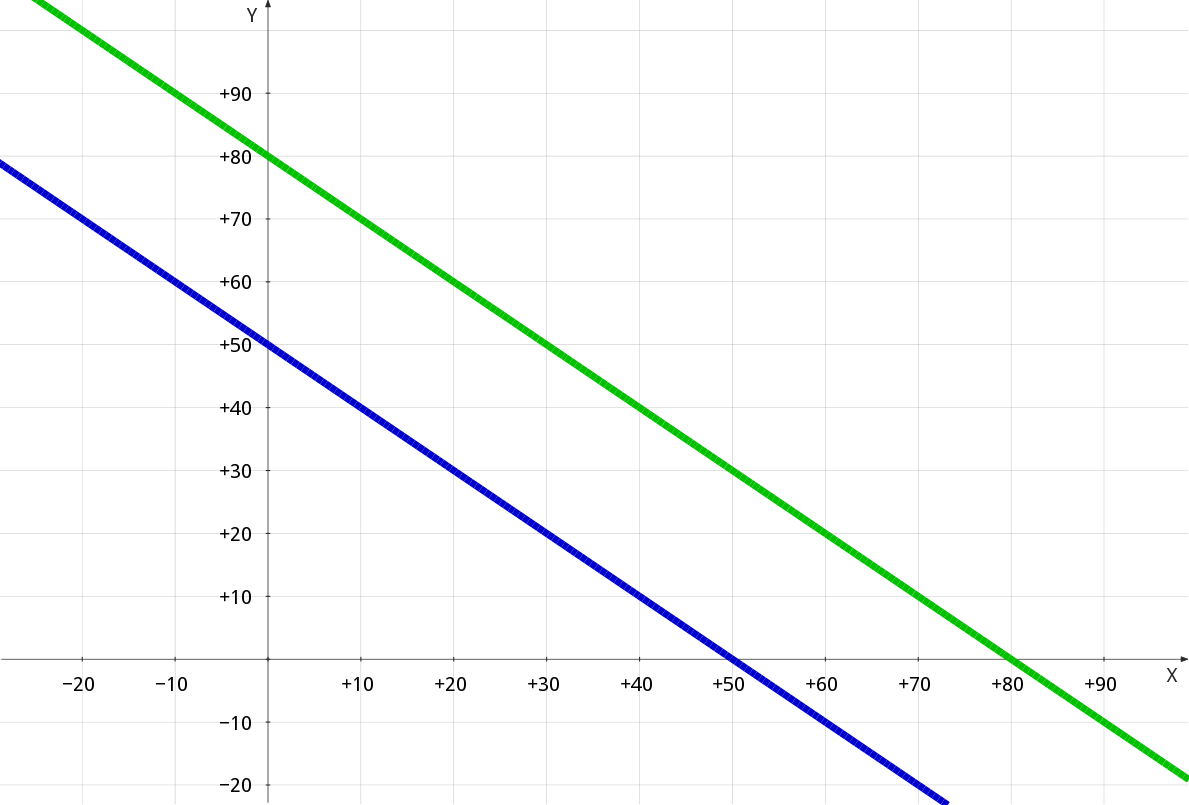
\includegraphics[width=8cm]{img/inconsistente.png}
	\end{center}
\end{frame}

\begin{frame}{Problemas?}
	$$\left\{ \begin{array}{r c r c l} x&+&y&=&80\\4x&+&2y&=&260\\x&-&y&=&20 \end{array} \right.$$
	\begin{center}
	   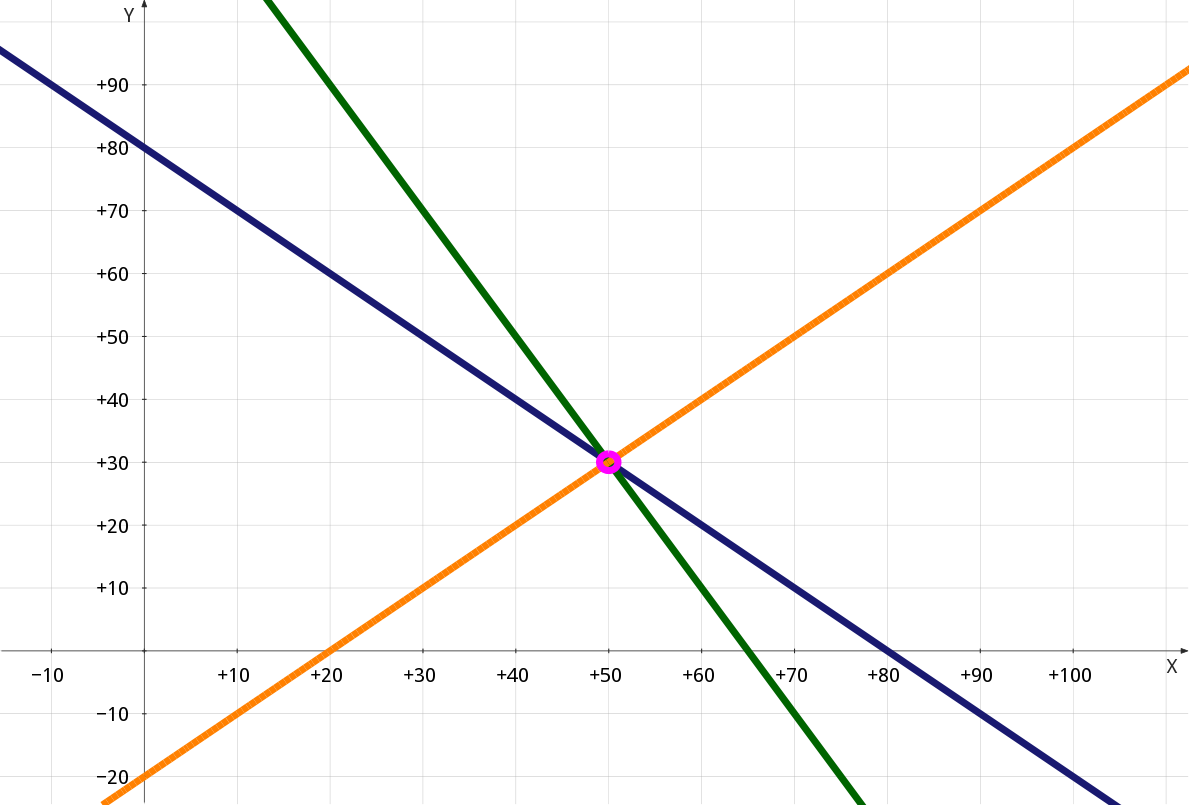
\includegraphics[width=8cm]{img/treseqs.png}
	\end{center}
\end{frame}

\begin{frame}{Problemas?}
	$$\left\{ \begin{array}{r c r c l} x&+&y&=&80\\4x&+&2y&=&260\\x&-&y&=&50 \end{array} \right.$$
	\begin{center}
	  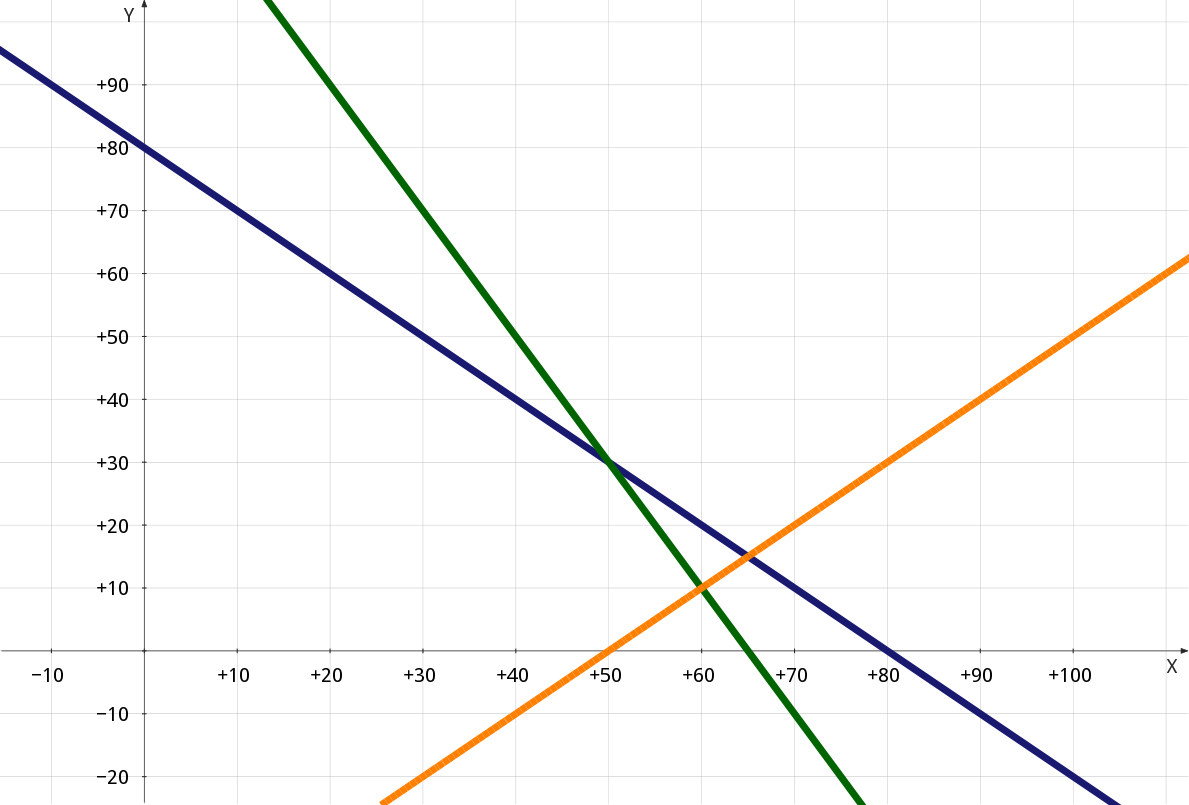
\includegraphics[width=8cm]{img/sobredeterminado.png}
	\end{center}
\end{frame}

\begin{frame}{Gráficos}
   Cada ponto no gráfico é dado por uma coordenada $(x,y)$, onde $x$ é um número real e $y$ é um número real associado a $x$ (como $y = f(x)$). Mas, não podemos representar a reta real (\emph{contínua}) no MATLAB. Por isso, precisamos pegar um vetor de pontos:
   $$x = (x_1, x_2, \ldots, x_n)$$
   e fazer o gráfico de $f$ apenas nestes pontos; o MATLAB ligará o resto. 
   \begin{center}
      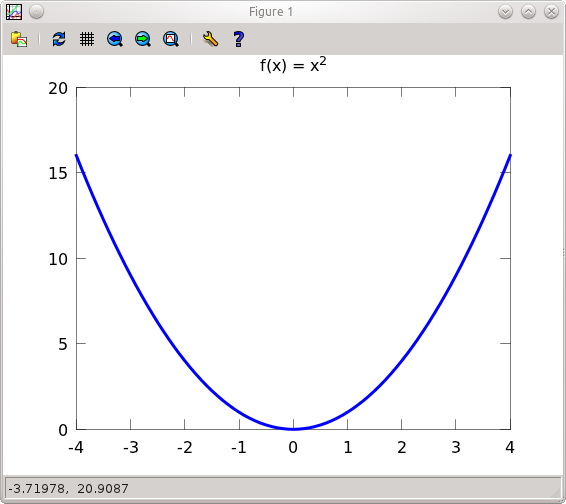
\includegraphics[width=4cm]{img/grafico_exemplo.png}
   \end{center}
\end{frame}

\begin{frame}
   \frametitle{Plot}
   O comando para fazer gráficos no MATLAB é 
   \begin{center}
      {\texttt{plot(x,y)}}
   \end{center}
   em que $x$ é um \emph{vetor} dos pontos onde a função será avaliada, e $y$ é um \emph{vetor} tal que $y_i = f(x_i)$.

   Exemplo: $f(x) = x^2$; 
   $$x = (0,0.1,0.2,0.3,0.4,0.5,0.6,0.7,0.8,0.9,1.0)$$
   $$y = (0,0.01,0.04,0.09,0.16,0.25,0.36,0.49,0.64,0.81,1.0)$$
\end{frame}

\begin{frame}{Gráficos}
  Para criar estes vetores, podemos usar os seguintes comandos:
  \begin{itemize}
  \item[{\texttt{>>}}] {\texttt{x = 0:0.1:1}}
  \item[{\texttt{>>}}] {\texttt{y = x\alert{.\^{}}2}}
  \item[{\texttt{>>}}] {\texttt{plot(x,y)}}
  \end{itemize}
  \vfill
  \emph{$x$ pode ser um vetor linha ou coluna.}
\end{frame}

\begin{frame}{Exemplo}
  Sistema Linear: 
  \begin{equation*}
    \left\{ 
    \begin{matrix} 
      x_1&+&x_2&=&8\\
      4x_1&+&2x_2&=&26 
    \end{matrix} 
    \right. \Leftrightarrow \left\{ 
    \begin{matrix} 
      x_2&=&8 &-& x_1\\
      x_2&=&13 &-& 2x_1
    \end{matrix} 
    \right.\Leftrightarrow 
    \begin{pmatrix}
      x_1\\x_2
    \end{pmatrix} = 
    \begin{pmatrix}
      5\\3
    \end{pmatrix}
  \end{equation*}
  \vfill
  \begin{itemize}
  \item[{\texttt{>>}}] {\texttt{x1 = 0:0.1:10}}
  \item[{\texttt{>>}}] {\texttt{plot(x1,8-x1)}}
  \item[{\texttt{>>}}] {\texttt{\alert{hold on}}}
  \item[{\texttt{>>}}] {\texttt{plot(x1,13-2*x1)}}
  \item[{\texttt{>>}}] {\texttt{\alert{hold off}}}
  \end{itemize}
\end{frame}

\begin{frame}{Opções do comando {\texttt{plot}}}
  \begin{itemize}
  \item[{\texttt{>>}}] {\texttt{help plot}}
  \end{itemize}
  \begin{columns}
    \column{7cm}{
      \begin{columns}
        \column{3cm}
        Estilos de linha:
        \footnotesize{%
          \begin{itemize}
          \item['-'] Linha contínua
          \item['.'] Pontos
          \item['+'] 
          \item['*']
          \item['o']
          \item['x']
          \item['\^{}']
          \end{itemize}
        }
        \column{3cm}
        Cor do gráfico:
        \footnotesize{%
          \begin{itemize}
          \item['k'] preto
          \item['r'] vermelho
          \item['g'] verde
          \item['b'] azul
          \item['m'] rosa
          \item['c'] azul claro
          \item['w'] branco
          \end{itemize}
        }
      \end{columns}
    }
    \column{5cm}{
      Exemplos:
      \begin{itemize}
      \item[{\texttt{>>}}] {\texttt{plot(x,y,'r*')}}
      \item[{\texttt{>>}}] {\texttt{plot(x,y,'m\^{}')}}
      \end{itemize}
      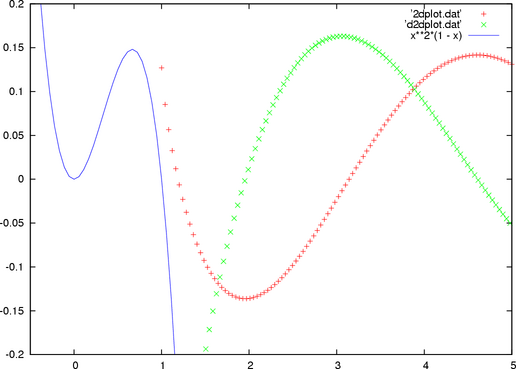
\includegraphics[width=4cm]{img/exemplo_tudo.png}
    }
  \end{columns}
\end{frame}
\end{document}
